\chapter{怎样寻找优质的教程}
\label{how-to-find-tutorials}

\begin{intro}
  在软件篇开始的时候我们就强调了,《Missing》从来不会是任何一款具体软件的教程。这是由这份教程的编写初衷决定的——每个人所需要掌握的软件都不一样,要学习的具体方面更是千差万别,《Missing》无法,也不可能成为一个人人都能取用的大杂烩。相反地,《Missing》在这里向大家介绍「怎样寻找优质的教程」。
\end{intro}

一份好的软件教程能帮助我们更快、更熟练地使用软件。今天,互联网上的内容多如牛毛,但像《Missing》这样用心编写的优质教程却少之又少。寻找优质软件教程,如同「沙里淘金」。这一部分将向大家介绍一些可能更容易找到优质教程的方法。

\section{利用好软件的官方文档}

在许多时候,软件的开发商会为自己的产品撰写文档。这些文档往往可以免费在互联网上获取到,而且相当权威和准确。将官方文档作为学习参考,不失一种不错的选择。

例如,如果你想学习 Excel 软件中「函数」部分的使用,那么可以查阅微软官方的 Excel 文档,例如图 \ref{MS_Excel_functions} 所示的\href{https://support.microsoft.com/zh-cn/office/excel-%E5%87%BD%E6%95%B0-%E6%8C%89%E7%B1%BB%E5%88%AB%E5%88%97%E5%87%BA-5f91f4e9-7b42-46d2-9bd1-63f26a86c0eb}{这一份}。

\begin{figure}[htb!]
  \centering
  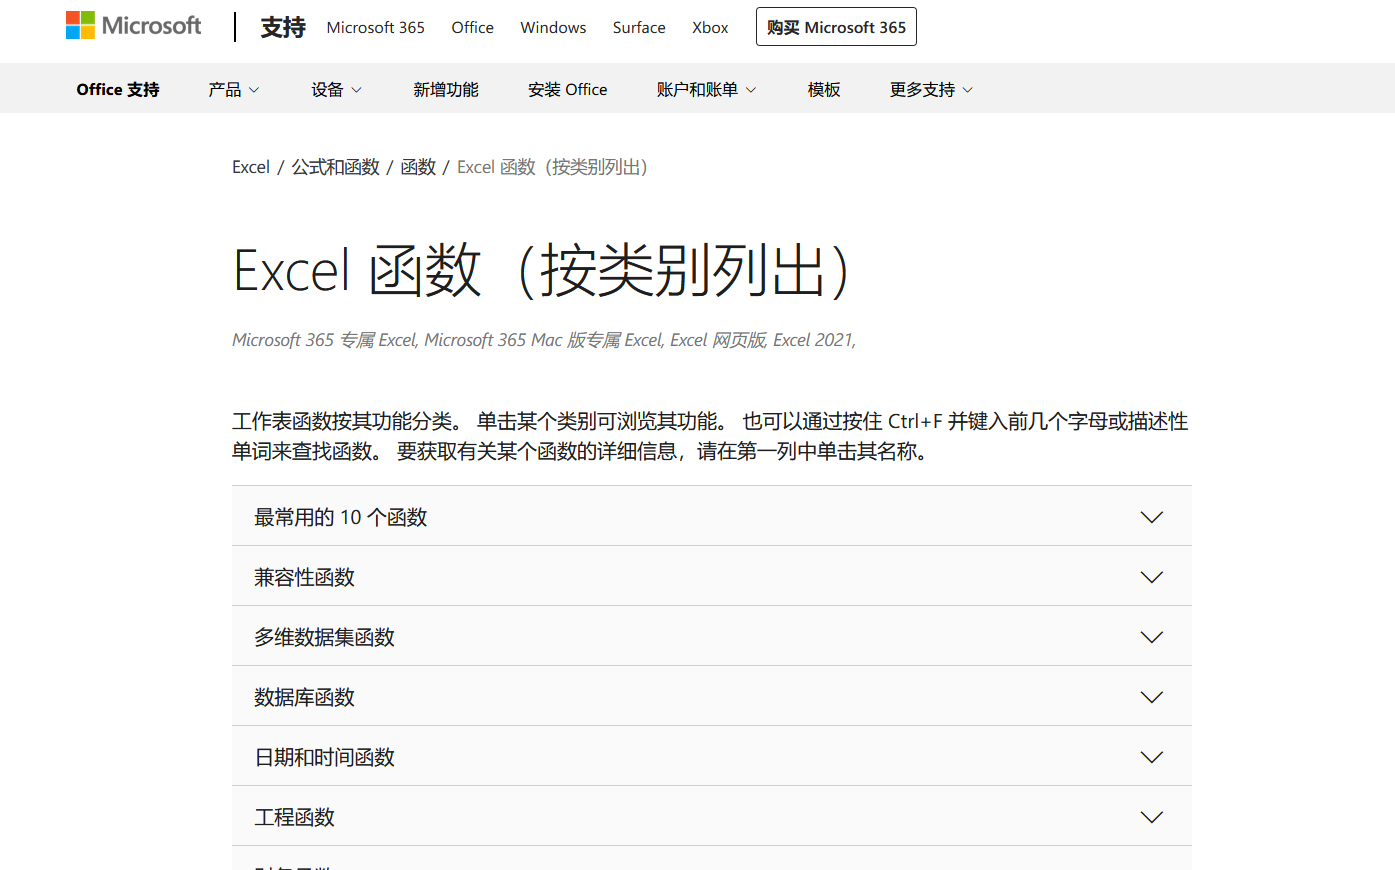
\includegraphics[width=12cm]{assets/MS_Excel_functions.png}
  \caption{微软官方的 Excel 函数文档}
  \label{MS_Excel_functions}
\end{figure}

这份官方文档不仅对每一个 Excel 函数都有介绍,并且还附上了各种使用例,因而比较容易学习。图 \ref{Excel_SUM} 和图 \ref{Excel_MATCH} 分别是 \verb|SUM| 和 \verb|MATCH| 两个函数的介绍中给出的例子与解释。

\begin{figure}[htbp]
  \centering
  \begin{minipage}{6cm}
    \centering
    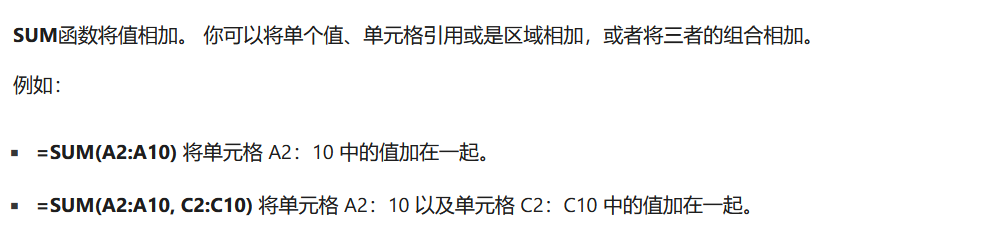
\includegraphics[width=5cm]{assets/Excel_SUM.png}
    \caption{Excel 函数 \texttt{SUM} 的使用说明}
    \label{Excel_SUM}
  \end{minipage}
  \qquad
  \begin{minipage}{6cm}
    \centering
    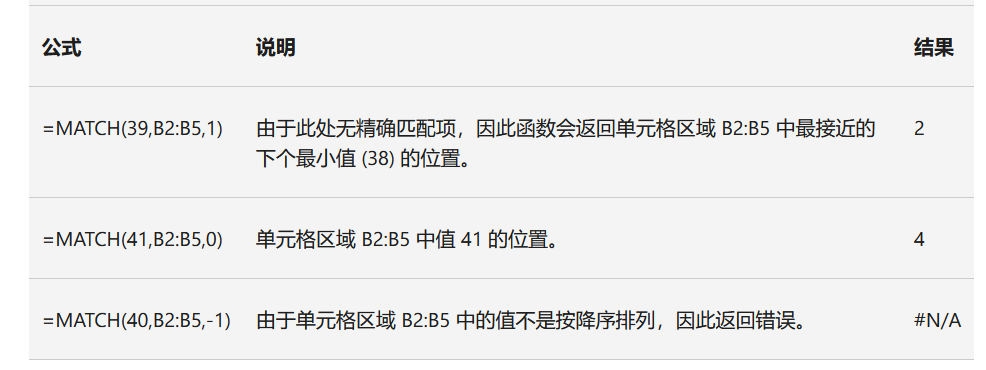
\includegraphics[width=5cm]{assets/Excel_MATCH.png}
    \caption{Excel 函数 \texttt{MATCH} 的使用说明}
    \label{Excel_MATCH}
  \end{minipage}
\end{figure}

又比如说,你想了解 Photoshop 的使用,那么 Adobe 官方也有制作一系列「新手向」的教程(甚至还有视频,带中文字幕,顺便附赠用到的素材),如图 \ref{PS_official_tutorial} 所示。

\begin{figure}[htb!]
  \centering
  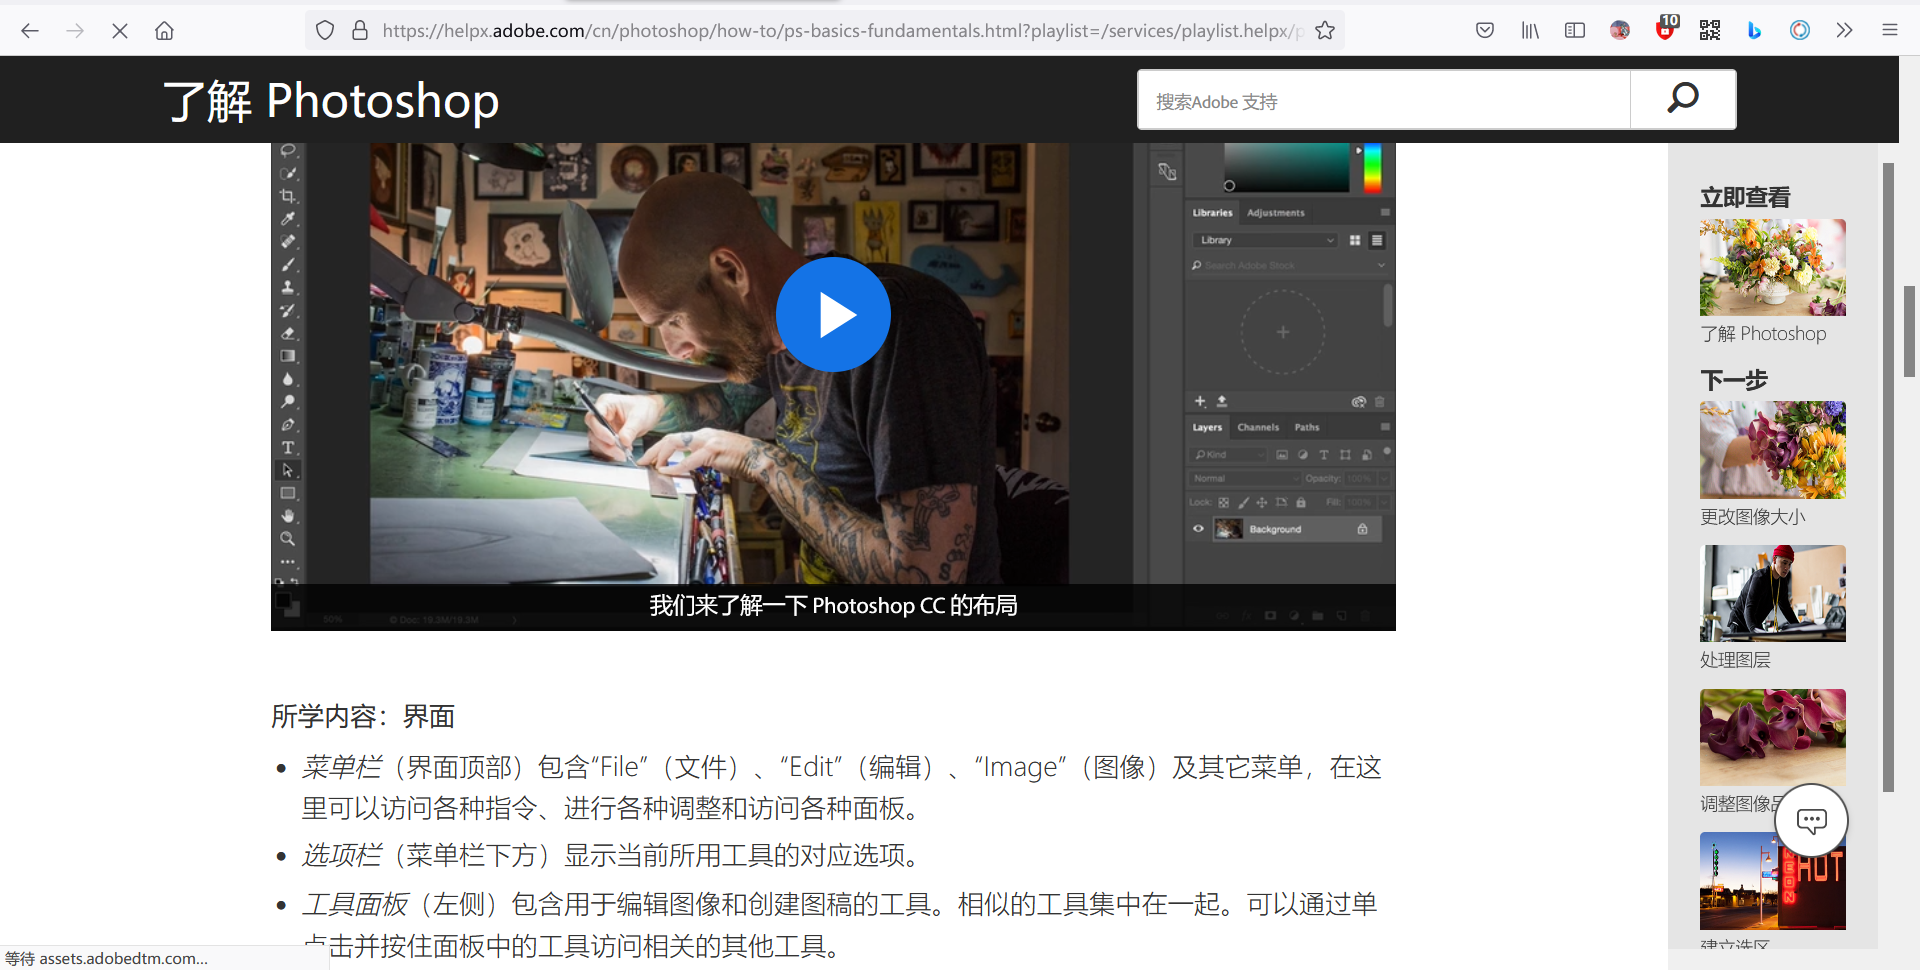
\includegraphics[width=12cm]{assets/PS_official_tutorial.png}
  \caption{Adobe 官方推出的 Photoshop 教程}
  \label{PS_official_tutorial}
\end{figure}

一般来说,我们可以通过访问软件的官方网站(不知道怎么找官网?请参看\nameref{software-installation}),并在官方网站寻找名为「帮助」或「支持」的栏目来查找官方文档 / 官方教程。此外,你也可以直接在网上搜索「<软件名>\ 官方文档」「<软件名>\ 帮助\ 支持」等来尝试直接寻找相关的官方文档。

然而,尽管官方文档在一些时候相当好用,但有时候软件厂商并没有公开相关软件的文档,又或者官方文档写得相当晦涩难懂,再或者官方文档没有中文版本。这时,我们就需要寻找那些其他的民间教程了。

\section{寻找优质教程的平台}

在\nameref{how-to-find-solutions}中,我们已经介绍了一些挑选教程的注意事项,如「关注更新时间」「警惕洗稿文」等。下面,我们会对中文互联网上常见的一些教程平台做一些介绍,并以推荐程度排序。

\subsection{各种「独立博客」}

在整个中文互联网上,有许许多多像笔者们一样的「独立博客」博主——所谓的「独立博客」,指的是有自己的网站(例如,《Missing》的网址是 \url{https://missing.criwits.top/},这个网址完全由我们自己控制,不隶属于任何一个其他的平台),只登载作者自己的文章的博客。经验上来说,这些独立博客的内容质量一般较高,因此我们将它们放在推荐的第一位。

比如,如果你想初步学习 \LaTeX{} 的使用,那么图 \ref{Liam_LaTeX_tutorial} 展示的\href{https://liam.page}{《始终》}博客上的《一份其实很短的 \LaTeX{} 入门文档》就是一个非常不错的选择。

\begin{figure}[htb!]
  \centering
  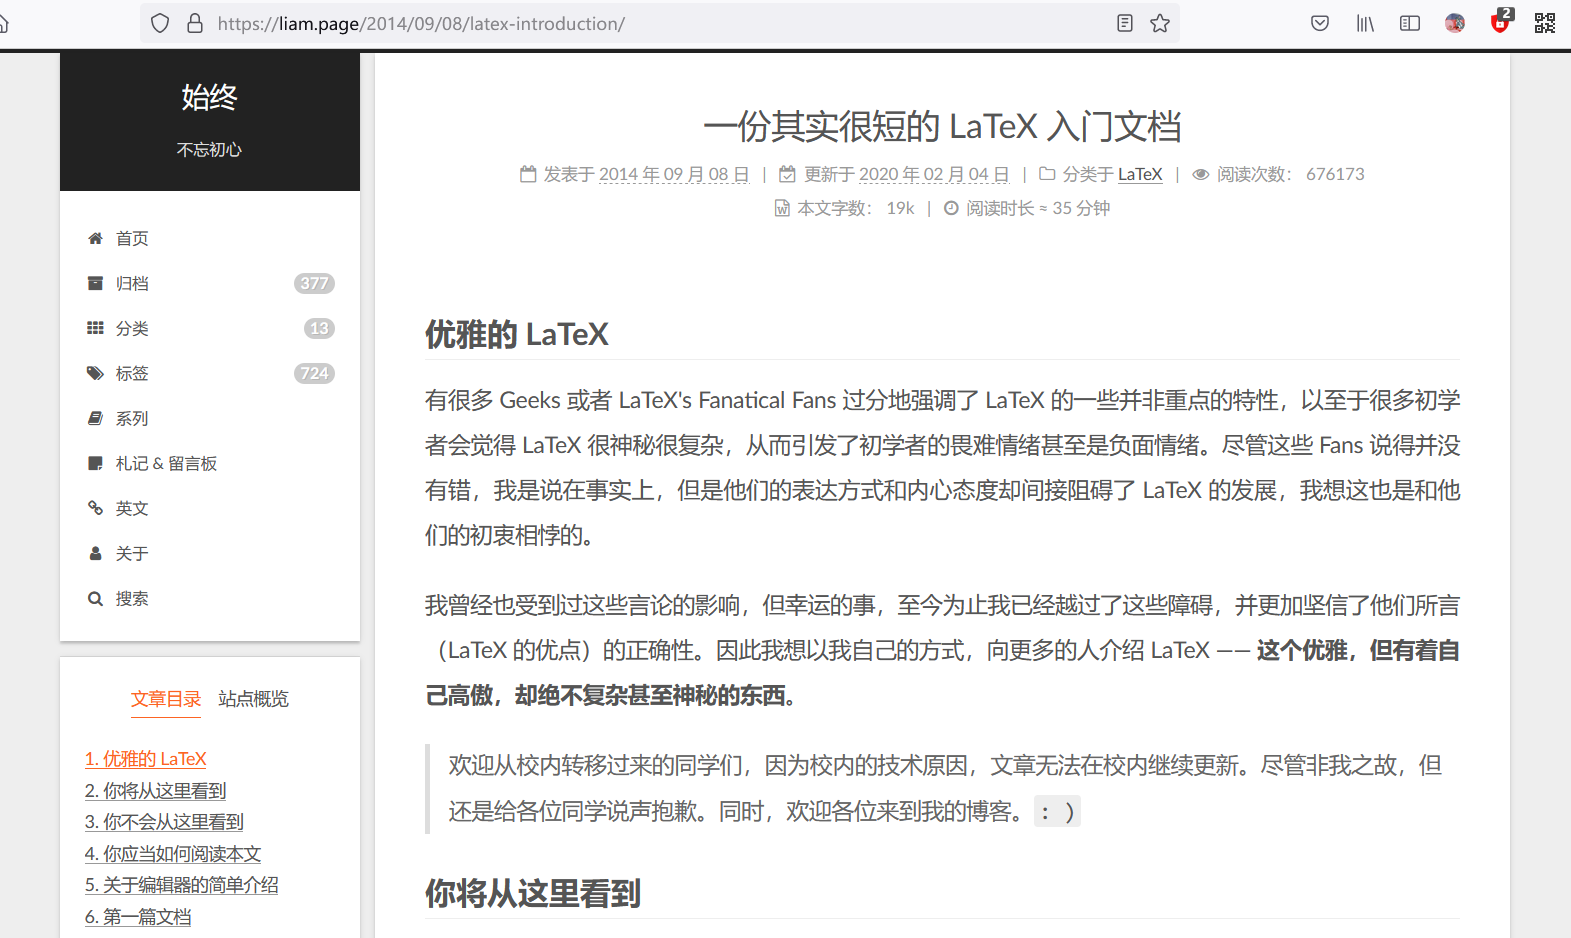
\includegraphics[width=12cm]{assets/Liam_LaTeX_tutorial.png}
  \caption{《一份其实很短的 \LaTeX{} 入门文档》}
  \label{Liam_LaTeX_tutorial}
\end{figure}

又比如,对于计算机相关方向的学习者,「廖雪峰」这个名字一定是不陌生的。图 \ref{Liao_Xuefeng} 展示的则是「廖雪峰的官方网站」,在那里你可以找到 Java、Python 等各种编程语言的入门教程。

\begin{figure}[htb!]
  \centering
  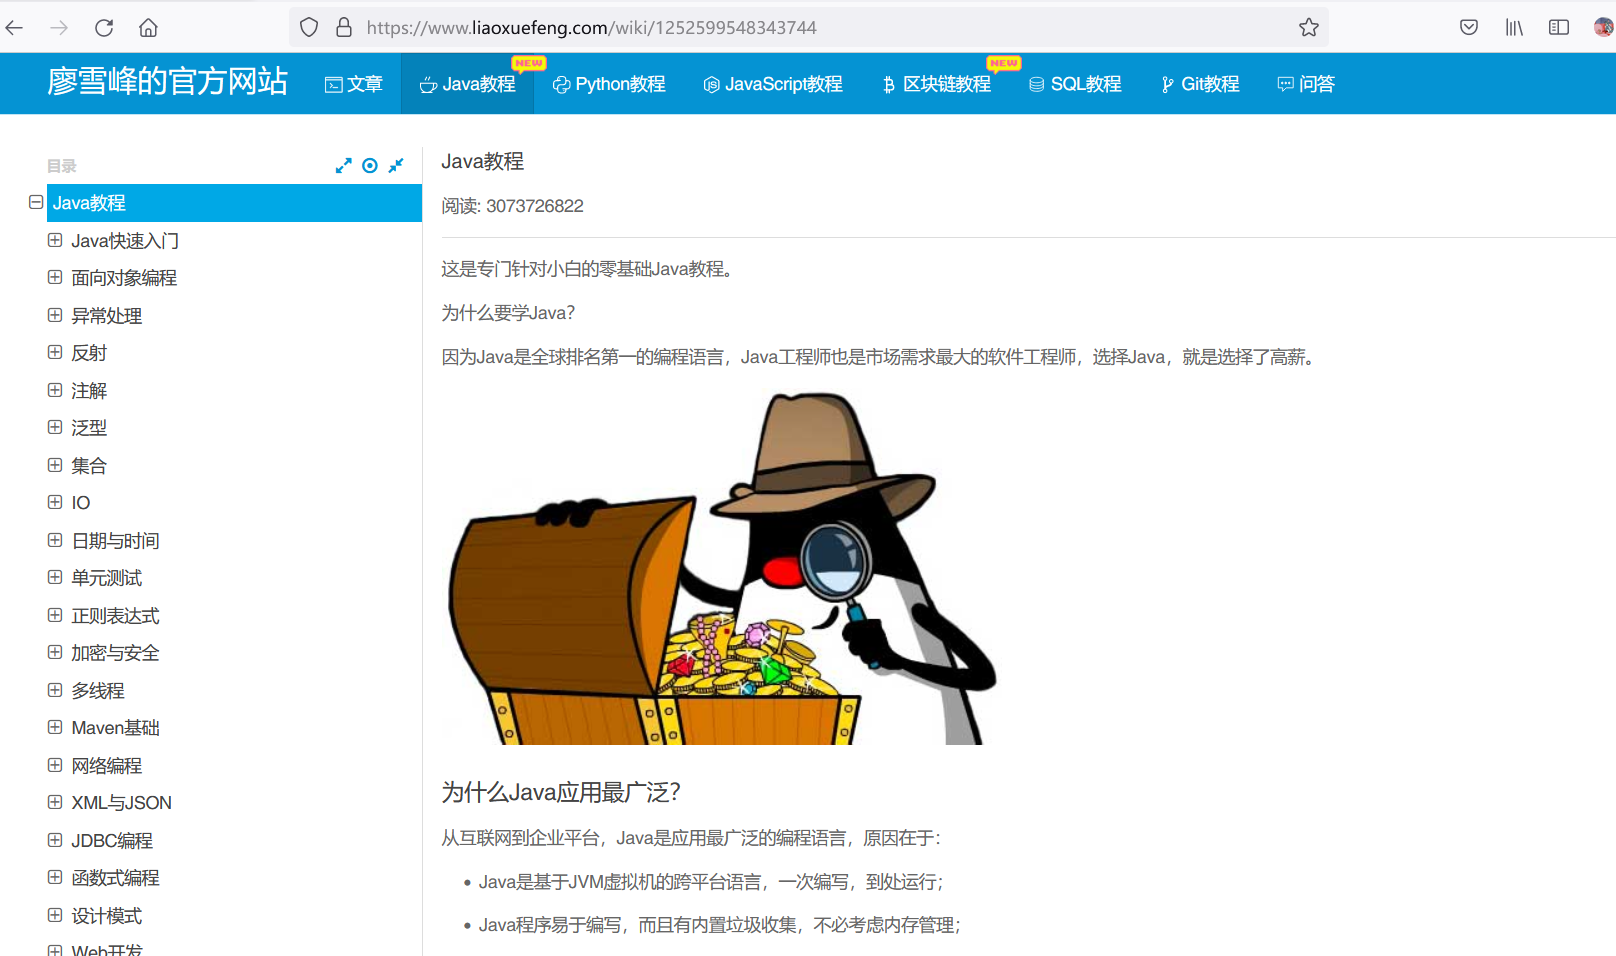
\includegraphics[width=12cm]{assets/Liao_Xuefeng.png}
  \caption{廖雪峰的官方网站}
  \label{Liao_Xuefeng}
\end{figure}

但将独立博客上的文章作为教程,缺点也很明显:首先,这样的内容通常「可遇不可求」——毕竟,这些博客分散在互联网的各处,能不能发现「宝藏」,全靠运气。其次,这些文章的覆盖面终究有限。博主们大都不是专门做教程的人,因而不太可能讲解到我们所需要学习的每一款软件。

受限于我们的知识积累,我们显然无法为大家总结出一个「优质博客列表」。大家可以在互联网上探索的过程中,不断地发现那些符合自己口味的博客和博主,并将它们分享给更多有需要的人。

\subsection{B 站、知乎、博客园及微信公众号等}

诸如 B 站(哔哩哔哩)、知乎和博客园等这样的内容产出平台,往往也有许多质量不错的各类教程供我们选择。例如,如果你想学习视频剪辑,那么在 B 站上有大量的相关软件教程可以观看;你想学习文字排版,在知乎上这方面的大佬数量也不少;至于学习各种开发类、技术类软件,那么博客园上的海量技术博客一定能满足你的需求。而在微信上,则有许多撰写或翻译各种优质软件教程的公众号,它们往往侧重于某一个学科领域(例如,软件开发或者建筑设计),时常推送相关软件的教程推文。

对于像 B 站和知乎这样的大型知识平台,我们可以直接在它们的搜索栏中寻找关键字,然后依据点击量或评论数等来轻松地筛选出更可能是优质内容的教程,如图 \ref{Bilibili} 所示。

\begin{figure}[htb!]
  \centering
  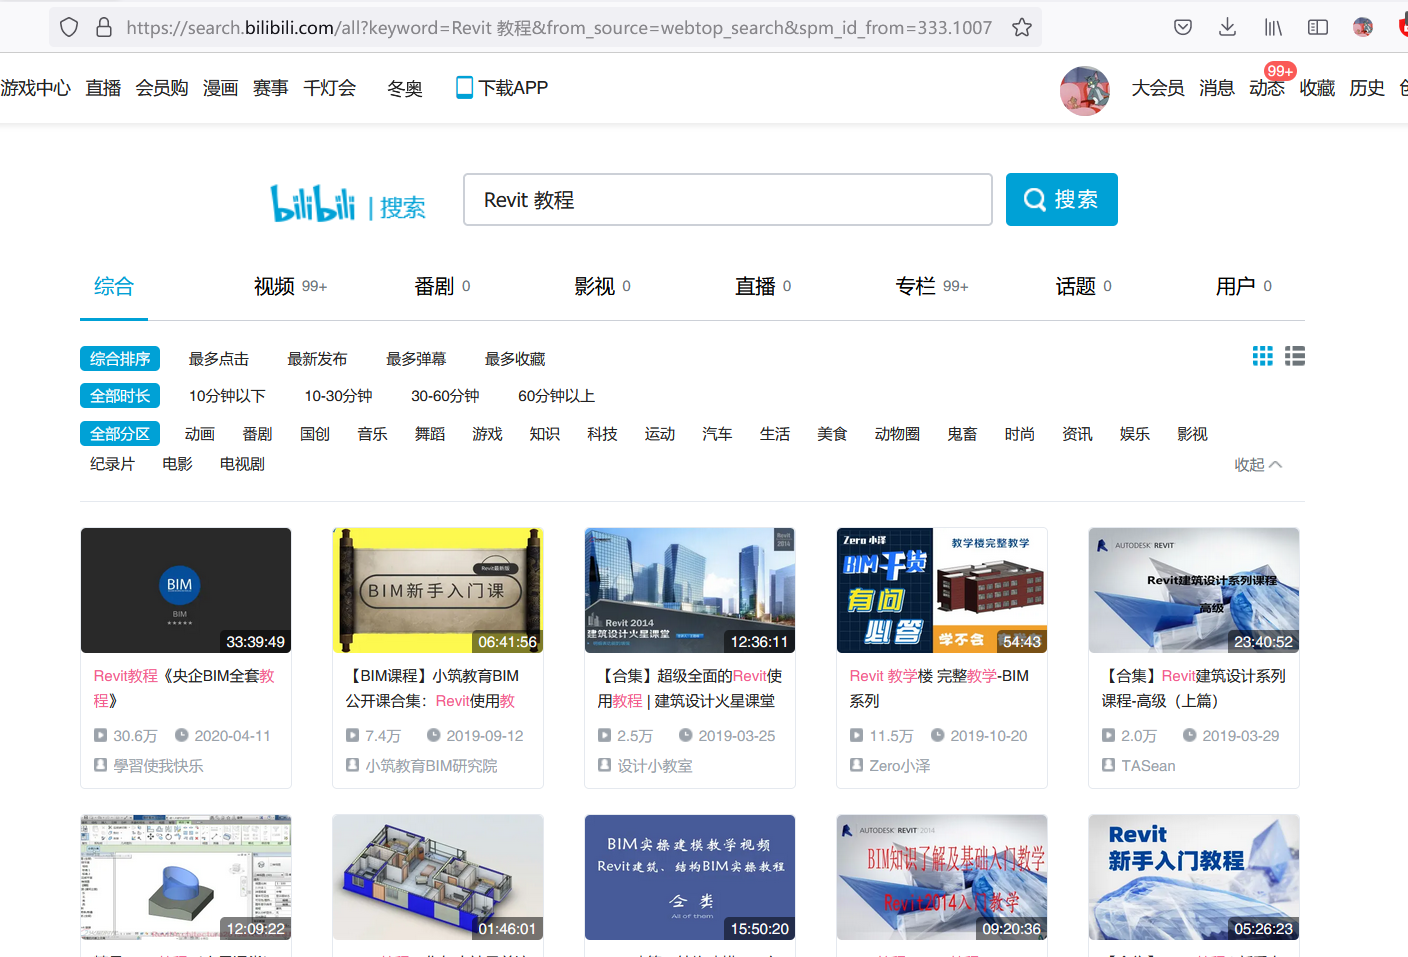
\includegraphics[width=12cm]{assets/Bilibili.png}
  \caption{在 B 站上搜索「Revit 教程」的结果}
  \label{Bilibili}
\end{figure}

而微信公众号——某种程度上它更像是低门槛的独立博客——则更多地依赖「口口相传」这样的方式来获得关注。如同我们在\nameref{software-installation}中提到的那种「软件分享」类的公众号,这里的「教程类」公众号也需要我们主动地「挖掘」,大家可以通过其他的途径去了解自己领域的优良公众号。

\subsection{CSDN、百度经验、百度知道等}

前面列出的那些平台,都有或多或少的参考价值,而像 CSDN、百度经验和百度知道这样的平台,则并不是我们推荐的选择。例如 CSDN,这个平台存在着非常严重的「洗稿」现象:一些人原文复制他人的文章——复制也就算了,还复制不全,抄来的东西都是错的。此外,像 CSDN 和腾讯云社区等平台还存在「假标题」的现象,部分页面吸引人点击却没有任何实质内容。甚至有些平台会出现「机翻国外网站教程」的现象,翻译质量嘛……不如不翻译。

\begin{figure}[htb!]
  \centering
  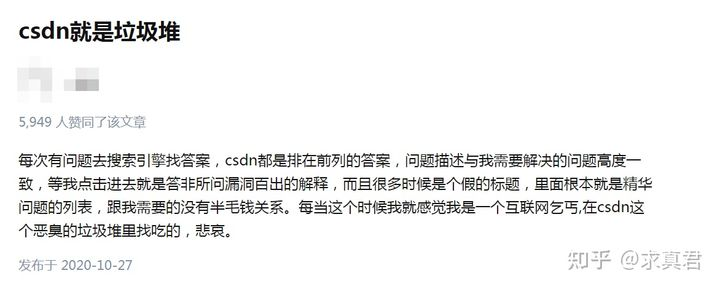
\includegraphics[width=10cm]{assets/CSDN_junk.png}
  \caption{网上关于 CSDN 平台的吐槽}
  \label{CSDN_junk}
\end{figure}

而像「百度知道」「百度经验」这种「烂大街」的平台,则更是充斥着无效的、过时的或错误的内容。尽管图 \ref{Baidu_zhidao} 是网友制作的恶搞图,但它却是对这些平台的一个实实在在的讽刺。

\begin{figure}[H]
  \centering
  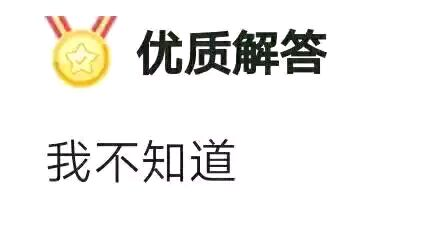
\includegraphics[width=4cm]{assets/Baidu_zhidao.png}
  \caption{百度知道「优质解答」:「我不知道」}
  \label{Baidu_zhidao}
\end{figure}

诚然,我们不能「一棒子打死」这些平台,这些平台上同样有值得参考和学习的文章。我们在这里强调它们的目的,是希望大家在查找教程时主动地有所侧重,并在选择教程时审慎行事。

\section{选择合适的搜索引擎 *}

想必大家一直以来都是使用「百度」作为自己的主要搜索引擎。诚然,作为中文互联网的早期企业之一,百度在中文搜索领域有着相当的技术积累;又由于一些国外企业「水土不服」,二十年来,百度都几乎「垄断」了国内搜索引擎的市场。

然而,今天的百度给我们带来的,除了便利,更多的是困扰。还记得\nameref{software-installation}中,我们演示搜索「WPS 下载」时,百度提供的整整一版的恶性广告吗?这些广告伴随着各种「洗稿文」「标题党」,为我们奉上了一场令人「大快朵颐」的中文互联网「盛宴」。

那我们就没有别的选择了吗?显然——不是。同样作为国际主流搜索引擎,\href{https://cn.bing.com/}{必应}不仅在国内可以正常、流畅地访问,还支持外文结果搜索,因而是我们相当推荐的搜索引擎之一。图 \ref{Bing_1} 是必应的搜索结果页。

\begin{figure}[htb!]
  \centering
  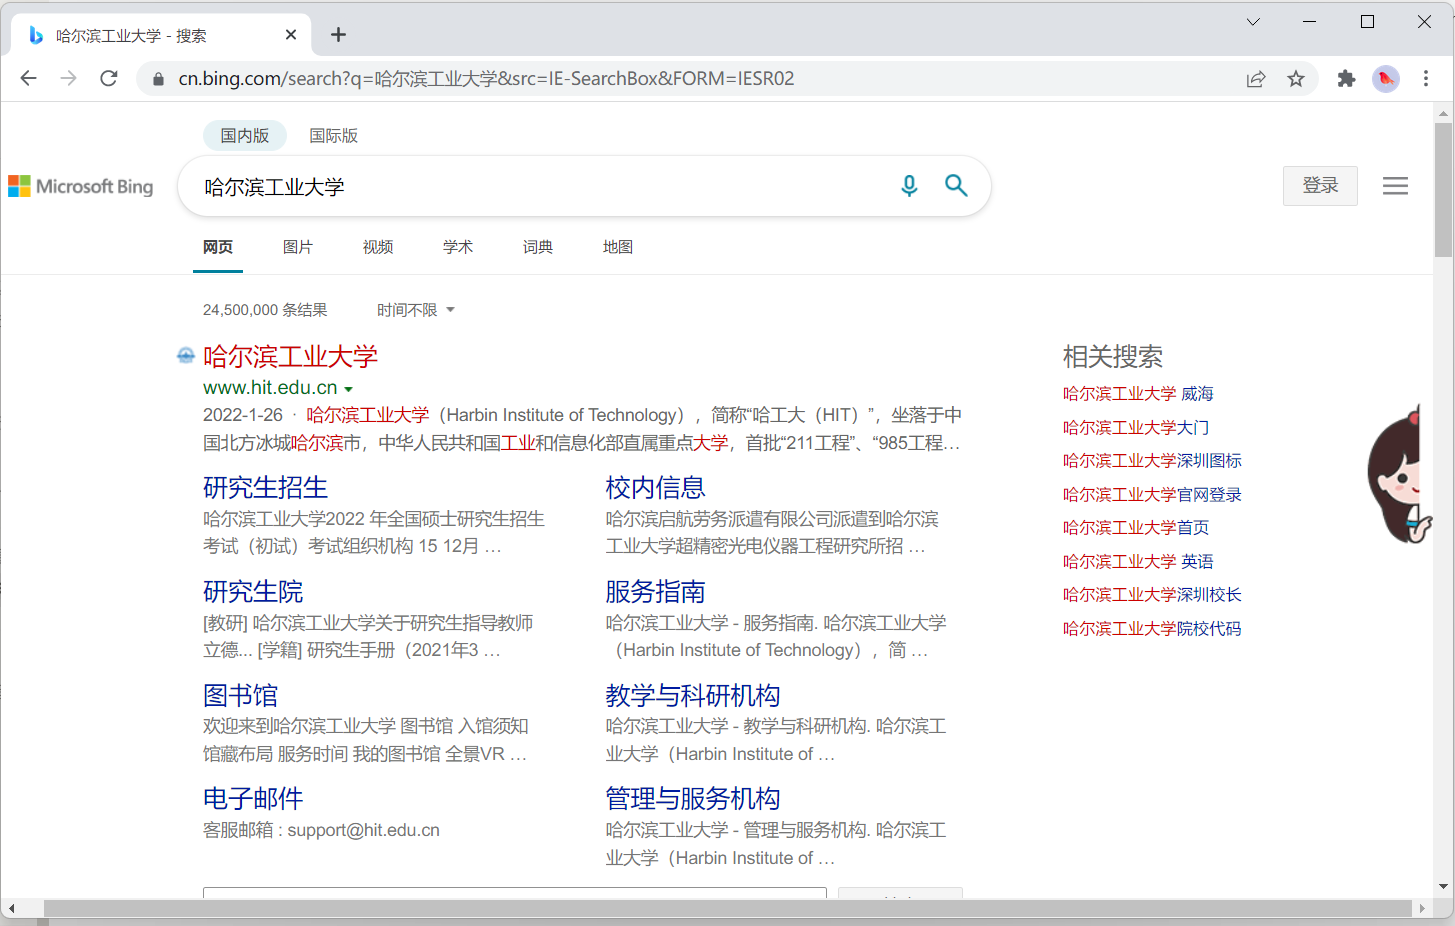
\includegraphics[width=12cm]{assets/Bing_1.png}
  \caption{必应的搜索结果页}
  \label{Bing_1}
\end{figure}

若你同样也忍受不了百度日渐增多的广告,那么或许必应是适合你的下一款搜索引擎。不妨尝试将必应设置为你的默认搜索引擎或主页。顺带说一句,必应每天都会更换一章首页封面图片(如图 \ref{Bing_2}),当做壁纸也是一个不错的选择哦!

\begin{figure}[htb!]
  \centering
  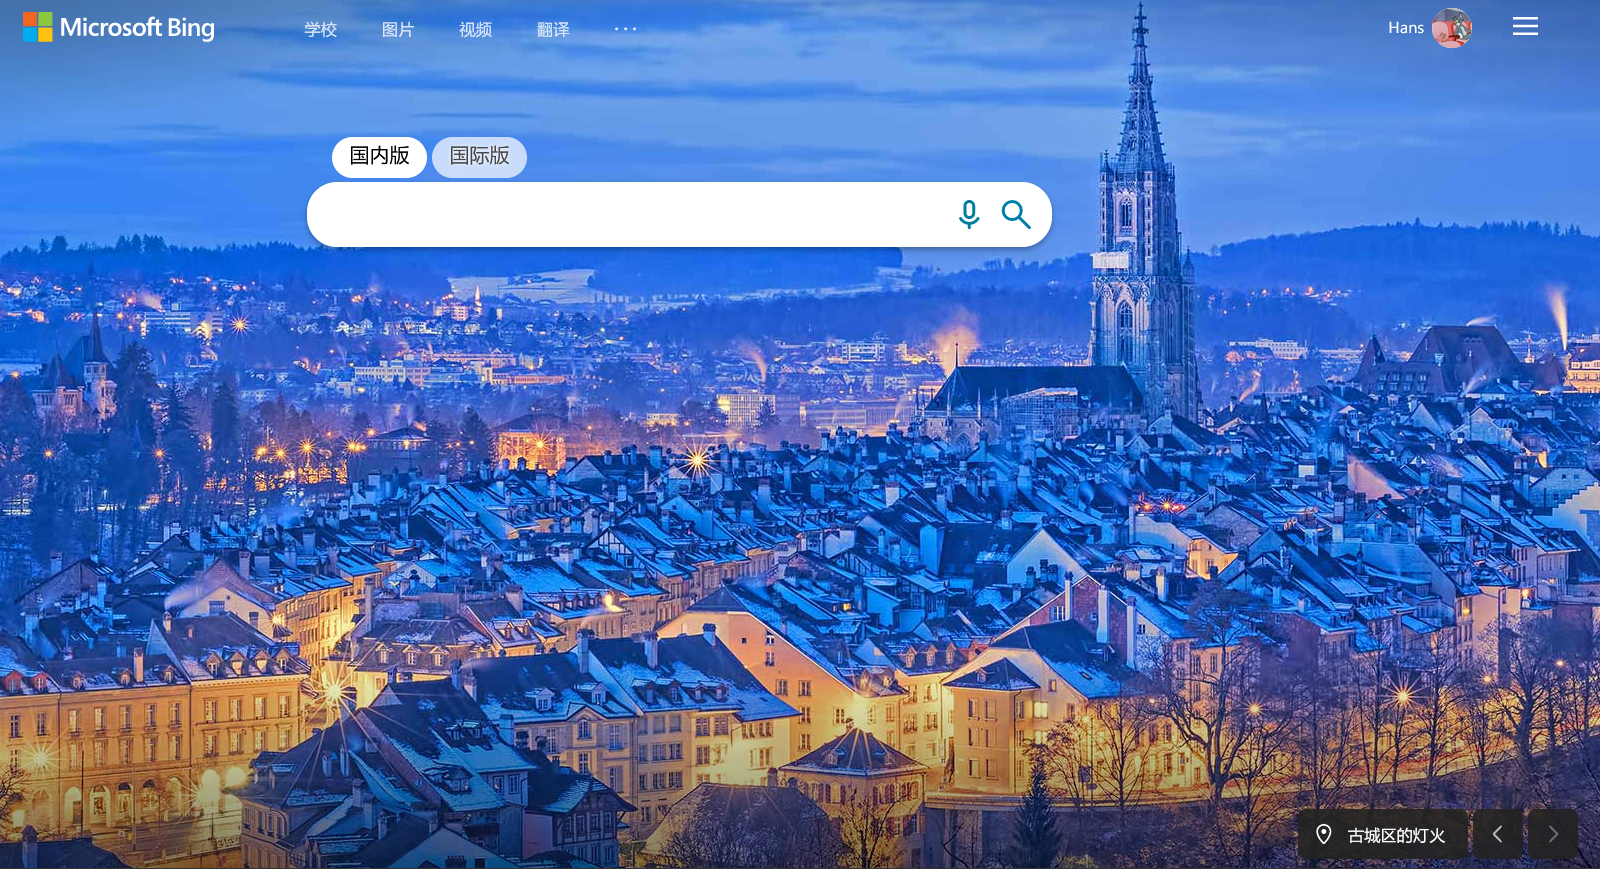
\includegraphics[width=12cm]{assets/Bing_2.png}
  \caption{必应首页,背景图片每天都会更新}
  \label{Bing_2}
\end{figure}

\practice

\begin{enumerate}
  \item 试着在网上寻找一篇来自独立博客的,你认为比较优质的教程(除了你现在正在看的)。
  \item 试着在文中介绍的那些互联网平台上查找你最近正在学或即将学习的软件的教程。
  \item 尝试一些除了百度之外的搜索引擎。
\end{enumerate}
